\chapter{Entwurf}
Um das benötigte Plug-in System zu realisieren, boten sich verschiedene
\first{Application Frameworks} an, die eine entsprechende Funktionalität
bereitstellen und somit als Programmbasis für die  Pipeline dienen konnten.
\index{Application Framework}
Die Wahl fiel hier auf das \first{OSGi Framework} \first{Equinox}, welches von
der \name{Eclipse Fundation} entwickelt wird und auch die Basis für die
Entwickungsumgebung \name{Eclipse} darstellt.
\index{Equinox}
\index{OSGi}
\index{OSGi Framework|see{OSGi}} 
\index{Eclipse}

\name{Eclipse Equinox} ist in Java geschrieben, was der Portierbarkeit der
Pipeline entgegenkommt. Ausserdem bietet die Framework-Architektur maximale
Modularisierung, wodurch sich Anwendungen auf \name{Equinox}-Basis durch
hervorragende Erweiterbarkeit und Skalierbarkeit auszeichnen.

\subsubsection{Das OSGi Framework}\label{chp:osgi}

Die \name{OSGi Alliance}, früher \enquote{\textit{Open Services Gateway
initiative}}, ist ein Zusammenschluß verschiedener Unternehmen, wie z.B. IBM,
Oracle oder Sun Microsystems.
Sie spezifiziert die \first{OSGi Service Platform}, eine Java-basierte
Softwareplattform, die nach einem \first{Komponentenmodell}
% footnote is von wikipedia !!!
\footnote{nach Gruhn und Thiel\citep{gruhn_komponentenmodelle_2000}:
\enquote{Ein Komponentenmodell legt einen Rahmen für die Entwicklung [..] von
Komponenten fest, der strukturelle Anforderungen hinsichtlich Verknüpfungs-
bzw. Kompositionsmöglichkeiten sowie verhaltensorientierte Anforderungen
hinsichtlich Kollaborationsmöglichkeiten an die Komponenten stellt.}}
organisiert ist.
\citep{wtherich_die_2008}
Einzelne Komponenten, sogenannte \first{Bundles}, können der Anwendung
dynamisch hinzugefügt und wieder entfernt werden ohne dass ein erneutes
Kompilieren oder Starten der Anwendung nötig ist.
Abhängigkeiten zwischen Bundles werden dabei automatisch aufgelöst; ein
intelligentes Versionsmanagement steht ebenfalls zur Verfügung.

Die \name{OSGi Service Platform} weisst ausserdem eine serviceorientierte
Architektur \footnote{Unter \first{serviceorientierte Architektur} oder auch
\first{dienstorientierte Architektur} versteht man ein Softwaredesign, dass
sich durch sogenannte Dienste oder auch Services auszeichnet. Diese können
appliktaions-global an einer Registry angemeldet und abgefragt werden. Sie
stellen dabei eine Schnittstelle zu bestimmten Funktionen bereit, ohne dabei
die zu Grunde liegende Implementierung preiszugeben.}
auf: 
Sie stellt eine globale Registry (\first{Service Registry})
bereit, an der Bundles \first{Dienste} bzw. \first{Services} anmelden und
abfragen können.

\subsection{Bundles}
Ein Bundle ist nach OSGi Spezifikation\citep{osgi_2009} eine technische Einheit
von Klassen und Ressourcen, die eigentständig in der Anwenung gestartet,
gestoppt, installiert und deinstalliert werden kann.
\index{Bundle}

Ressourcen und Klassen eines Bundles können anderen Bundles bereitgestellt
werden. Dazu müssen sie vom bereitstellenden Bundle explizit exportiert werden
und durch das nutzende Bundle explizit importiert werden. Jedes Bundle stellt einen
Bundlenamen, der üblicherweise von der enthaltenen Paketstruktur
abgeleitet wird, sowie eine Versionsnummer bereit. Aus diesen beiden Komponenten
wird dann eine eindeutige Identifizierung des Bundles generiert.
So ist es beispielsweise möglich, ein und das selbe Bundle in unterschiedlichen
Versionierungen zu installieren.

Über die \first{MANIFEST.MF}, die ohnehin in jedem Jar-File vorhanden ist, wird
das Bundle neben dem Namen und der Version mit weiteren Meta-Informationen, wie
importierte und exportierte Pakete oder Lauzeitumgebung, ausgestattet.
\index{MANIFEST.MF}

Jedes Bundle ist innerhalb des Frameworks mit einem eigenen Class-Loader
ausgestattet, über welchen ausschliesslich die Bundle-eigenen Klassen geladen
werden. Auf diese Weise sind die einzelen Bundles strikt voneinander getrennt und die
Import-Export-Beziehungen zwischen den Bundles können explizit gesteuert
werden. 
Neben anderen Vorteilen, wie etwa das Installieren des selben Bundles in
unterschiedlichen Versionen, wird auf diese Weise das vollständig
dynamische Hinzufügen und Entfernen von Bundles erst ermöglicht, da der
Class Path des Class Loaders nach dessen Instanziierung nicht mehr verändert
werden kann.
\citep{wtherich_die_2008}
% selbe version 17
% importieren, exportieren 13,79
% class loading 89
% MANIFEST.MF 21
% lebenszyklen 23,55
% unterschied Bundle / Plug-In 41
\paragraph{Services} % 93
Das OSGi Framework stellt gemäß der serviceorientierten Architektur eine
zentrale, bundleübergreifende \first{Service Registry} bereit, an der
sogenannte \first{Services} angemeldet und abgefragt werden können.
\index{Service Registry}
Ein Service ist in diesem Fall ein simples Java-Objekt, typischerweise ein
Interface, das unter dem Interface-Namen und einer optionalen Beschreibung an
der Registry angemeldet wird.
Der Zugriff auf die Registry kann durch jedes beliebige, im
Framework geladene Bundle erfolgen. Der Zugriff kann hier aktiv oder passiv
erfolgen.
\index{Bundle}

Bei einem aktiven Zugriff, also der Registrierung eines Services durch ein
Bundle, wird technisch gesehen ein Service-Namen, sowie eine Beschreibung des
Services an der Service Registry hinterlegt. Der Service-Name ist üblicherweise
der voll qualifizierende Klassenname des Service Interfaces, die Beschreibung
des Service ist eine Sammlung von Strings, die eine entsprechende Beschreibung
der bereitgestellten Funktion beinhalten.
\index{Service Interface}

Bei einem passiven Zugriff durch ein beliebiges Bundle, also dem Abfragen eines
Service über dessen Namen oder Beschreibung, liefert die Registry eine
Referenz auf das entsprechende Interface zurück.
Über diese Referenz auf das Service Interface kann nun die Funktionalität, die
dieses Interface bereitstellt, genutzt werden, ohne dass hierbei bekannt ist,
wie diese Funktionalität implementiert ist, oder welches Bundle diese
bereitstellt.

Durch die dynamische Modularisierung des OSGi Frameworks können Services zur
Laufzeit \enquote{kommen und gehen}. Es liegt in der Verantwortung des
nutzenden Bundles, auf die aktuelle Verfügbarkeit des Service entsprechend zu
reagieren.

Die \first{OSGi Service Platform} enthält aufbauend auf das OSGi Framework eine
Reihe von \first{Standard Services}, mit denen häufig wiederkehrenden
Problemstellungen begegnet werden kann. So steht beispielsweise ein Log-Service
zur Verfügung, über den Bundles Nachrichten absenden und empfangen können.
Desweiteren sind über die Standard Services auch Funktionenen zur
Benutzerverwaltung, HTTP oder Datenbankanbindung realisiert.
\index{OSGi Service Platform}
% Standard Services 13,25
\citep{wtherich_die_2008}

\begin{figure}[htbp]
	\begin{center}
		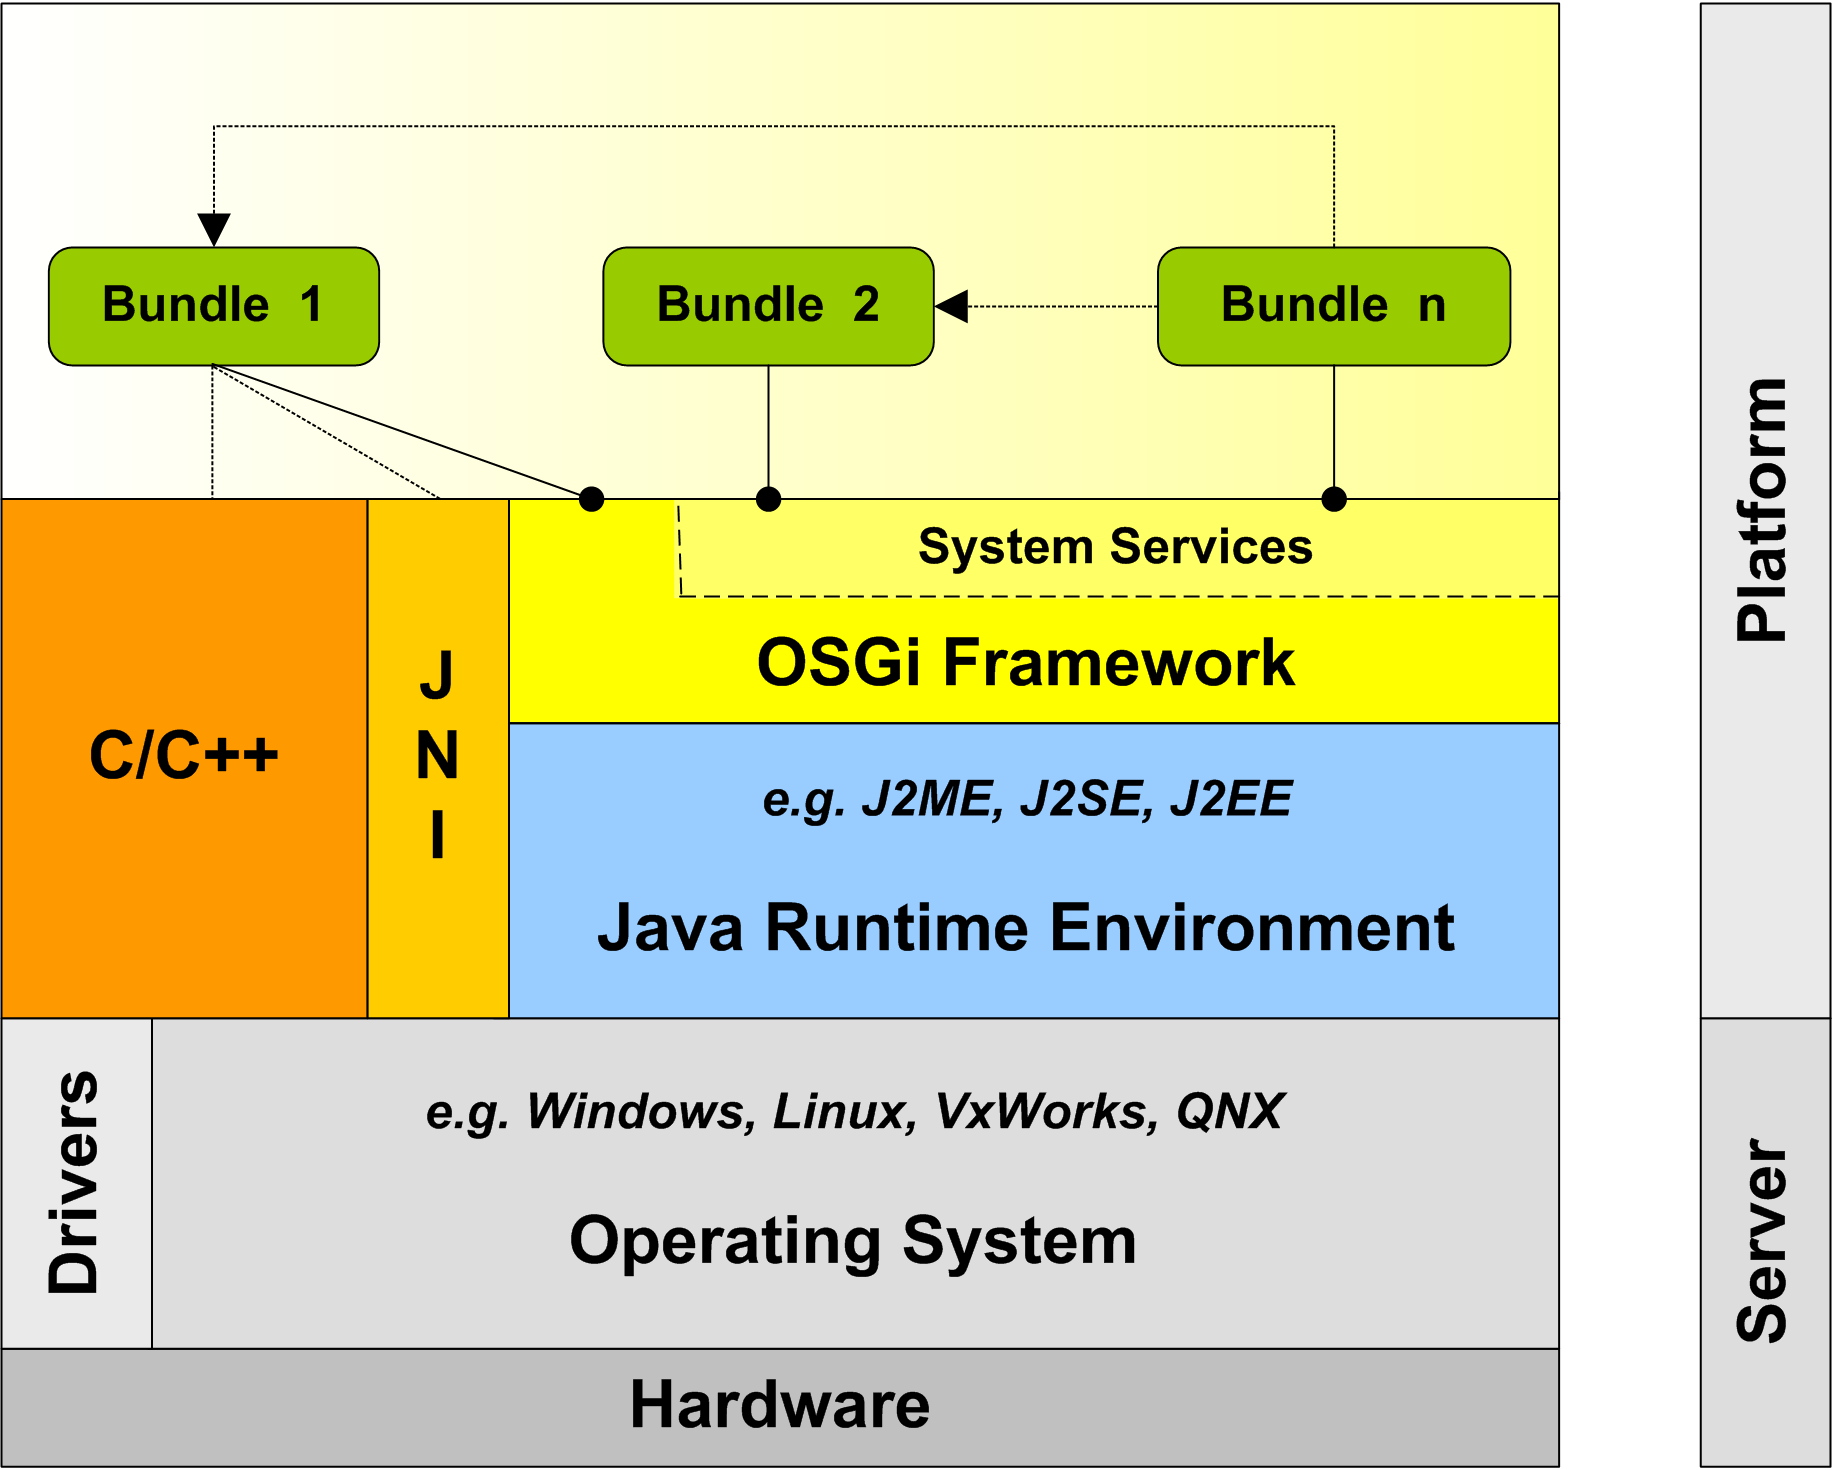
\includegraphics[scale=1.3]{pics/osgi_layer.png}
	\caption[OSGi Schichtenmodel]{
	\textbf{OSGi Schichtenmodel}
	}
	\end{center}
	\label{fig:osgi_layer}
\end{figure}

Die serviceorientierte Architektur der Pipeline wird also durch das
\name{OSGi Framework} diktiert und stellt somit die unterste Schicht der
Architekturabstraktion der Pipeline dar.


\section{Design}
Die Architektur der Software soll sich durch verschiedene Abstraktionebenen
darstellen lassen. \todo{hier könnte es etwas mehr sein}

\subsection{Pipes and Filters}
Die höchste Abstraktion stellt das \first{Pipes and
Filters}-Patten dar:
\footnote{\todo{pipes and filters}}
\index{Pipes and Filters}

\begin{figure}[htbp]
	\begin{center}
		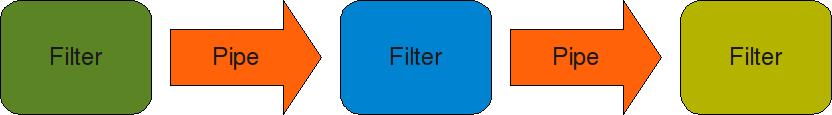
\includegraphics[scale=0.7]{pics/pipesFilter3.png}
	\caption[Pipes and Filter]{
	\textbf{pipesFilter.}
	something}
	\end{center}
	\label{fig:pipesFilter}
\end{figure}

Die zu annotierende Sequenz wird schrittweise durch verschiedene \first{Filter}
bearbeitet. Jeder Filter, der in der Pipeline vorhanden ist, wird dabei das
entgültige Ergebnis der Annotation durch seine spezifischen Ergebnisse
erweitern.

Der Input eines Filters besteht dabei zum einen aus der zu
annotierenden Sequenz selbst, zum anderen aus einem zentralen Datenobjekt, in
dem alle gewonnenen Ergebnisse abgespeichert werden.
Ein Filter kann dabei auch auf die Ergebnisse eines anderen
Filters angewiesen sein. Die Reihenfolge der Filter innerhalb der Pipeline wird
somit durch die spezifischen \first{execution preconditions}
\footnote{\todo{execution precondition}} aller Filter festgelegt.
\index{Filter}
\index{execution precondition}

Es ist davon auszugehen, dass die Ausführung einzelner Filter mitunter sehr
zeitintensiv sein wird. Ausserdem soll Nutzen aus dem im Institut installierten
\first{LSF} gezogen werden. Daher wird eine rein sequenzielle Abfolge der
Filter, wie es das Entwursmuster suggeriert, vermieden werden.
Stattdessen kann die Ausführung einzelner Filter parallel erfolgen.
Sind zu einem Zeitpunkt die execution preconditions mehrerer Filter erfüllt,
werden alle sofort zur Ausführung gebracht.
\index{Platform LSF}

Die Pipeline soll möglichst leicht konfigurierbar sein und sich an
individuelle Bedürfnisse anpassen lassen.
Vor diesem Hintergrund soll die Pipeline die veränderbaren Steps und das
statische \enquote{Ausführungsgerüst} vollständig entkoppeln. Beim Starten der
Pipeline soll diese an einem bestimmten Ort (lokales Verzeichnis oder
entferntes Repository) nach vorhandenen Steps suchen und diese in der Pipeline
installieren.

Die \name{Filter} des \name{pipes and filters} pattern sind somit aus der
eigentlichen Anwendung herrausgelöst. Sie sind über eine generische
Schnittstelle repräsentiert, deren Implementierung zur Kompilierzeit nicht
bekannt ist.

\begin{figure}[htbp]
	\begin{center}
		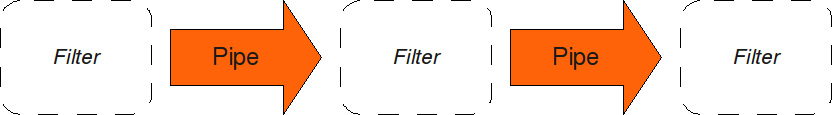
\includegraphics[scale=0.7]{pics/pipesFilter21.png}
	\caption[Pipes and Filter 21]{
	\textbf{pipesFilter 21.}
	something}
	\end{center}
	\label{fig:pipesFilter21}
\end{figure}

Die Pipeline teilt sich so in zwei Teilkomponenten:
Die \enquote{dynamischen Stepss} und das \enquote{statisches Ausfürhungsgerüst}.
Diese Anordnung legt eine weitere Abstraktionsebene nahe, nämlich das
\first{Client-Server-Modell}.
\footnote{\todo{Client-Server-Modell}}
\index{Client-Server-Modell}

\subsection{Client-Server-Modell}
Die \first{Pipes} des \name{pipes and filters} Pattern werden zu einem
\first{Server} zusammengefasst und bilden das {statische Ausführungsgerüst}.
Ein \first{Client} ist ein \first{Filter} des \name{pipes and filters} Pattern.
Die einzelnen Clients sind dynamisch und somit nicht Teil der
statischen Kernanwenung.
\index{Filter}
\index{Step}
\index{Client}
Es können sich beliebig viele Clients am Server anmelden, wodurch die
eigentliche Pipeline aufgebaut wird.
\todo{hmmhmm}

\subsubsection{Server}
Die Anforderungen an den Server gliedern sich in zwei Teilbereiche:
\begin{description}
\item[Organisation und Synchronisation der Client Ausführung]
Die Ausfürhrung der angemeldeten Steps kann sequenziell oder
parallel erfolgen, je nachdem, welche \first{execution preconditions} für den
jeweiligen Step erforderlich sind und ob die zur Ausführung benötigten Daten eventuell erst
durch einen anderen Step bereitgestellt werden müssen. Vor der eigentlichen
Ausführung wird der Server somit zum einen die \name{execution preconditions}
prüfen, zum anderen, ob der Step überhaupt zur Ausführung
gebracht werden muss, oder ob die zu erwartenden Ergebnisse bereits in selber
oder in anderer Form vorhanden sind.
\item[Datenverwaltung] Die Ergebnisse der einzelnen Steps werden zentral durch
den Server verwaltet.
Zum einen synchronisiert der Server die Zugriffe auf die Daten, zum anderen
werden diese persistiert, um bei einer gewollten oder ungewollten Unterbrechung
der Pipeline Datenverlust zu verhindern.
\end{description}

\subsubsection{Client}
Auf der Clientseite stehen die einzelnen \first{Filter} der Pipeline, im
folgenden \first{Steps} genannt \todo{hmmm}. Jeder Step soll technisch
gesehen einem oder mehreren OSGi-Bundles entsprechen.
\index{Step}
\index{Filter}
\index{Client}
\index{Bundle}
\index{OSGi-Bundle}
Wird das Bundle durch das OSGi-Framework gestartet, soll sich der Step am Server
anmelden. Der Step stellt dabei entsprechende \name{call-back-Methoden} für die
eigentliche Ausführung, Überprüfung der \name{execution preconditions} und
Ähnlichem bereit.
\index{Server}
\index{OSGi Framework}
\index{call back method}
Wann diese Methoden aufgerufen werden, obliegt so allein
dem Server.
Als Prameter der call back methoden wird die Sequenz, sowie das zentrale
Datenobjekt, im Folgenden \first{Data bean} \todo{hmmm} genannt,
übergeben.

\begin{figure}[htbp]
	\begin{center}
		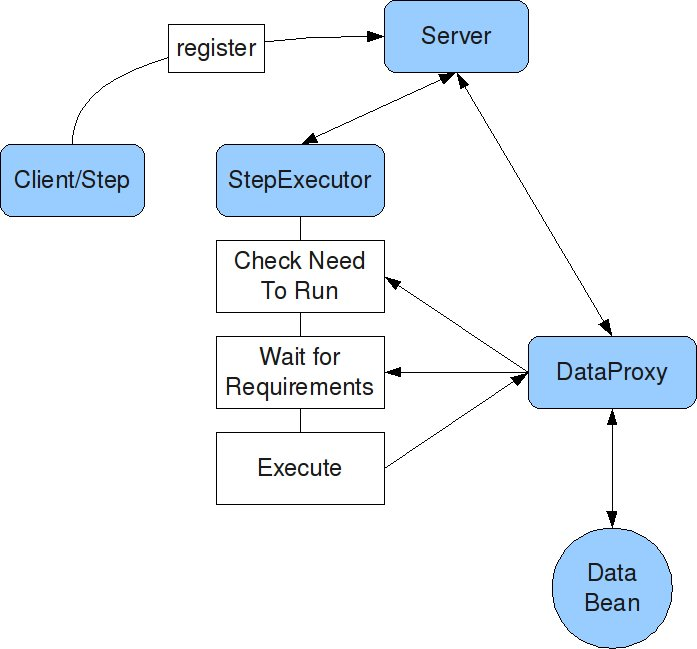
\includegraphics[scale=0.6]{pics/programOrganisationOverview3ScaledWithAlpha.jpg}
	\caption[Design 1]{
	\textbf{Design 1.}
	something. \todo{Teilung von Server hier noch nicht erwähnt. Evtl. Teil der
	Umstzung}}
	\end{center}
	\label{fig:programOrganisationOverview3ScaledWithAlpha}
\end{figure}

\section{Genvorhersage}
\todo{\dots}






 
